\chapter{Seguridad en NFC}\label{ch:seguridad}
En este capítulo trataremos temas relacionados con la seguridad en las tarjetas NFC. Analizaremos vulnerabilidades y los métodos más comunes y eficaces para securizar los equipos NFC.
\clearpage
\section{Justificación}
Como hemos visto en el apartado anterior de usos, muchos de estos sistemas son utilizados como monedero, por lo tanto, corromper el sistema significaría acceder al dinero del portador del dispositivo.\par
En sistemas de identificación, falsificar la identidad de un directivo de la empresa, podría conceder al hacker permisos indeseados para los intereses de la empresa. Por lo tanto, debido al tipo de información que tienen estos equipos, garantizar la seguridad es una prioridad.
\section{Amenazas}
Las amenazas más comunes de los sistemas NFC son:
\begin{itemize}
	\item Eavesdropping (Escucha)
	\item Skimming (Clonado)
	\item DoS (Denial of Service)
	\item Modificación de datos
	\item Inserción de datos
	\item Man-in-the-middle
\end{itemize}
%-----------
\subsection{Eavesdropping}
La técnica de eavesdropping consiste en estar escuchando las conexiones de la víctima y el receptor sin llegar a hacer nada con los paquetes.\\

\begin{figure}[!h]
	\centering
	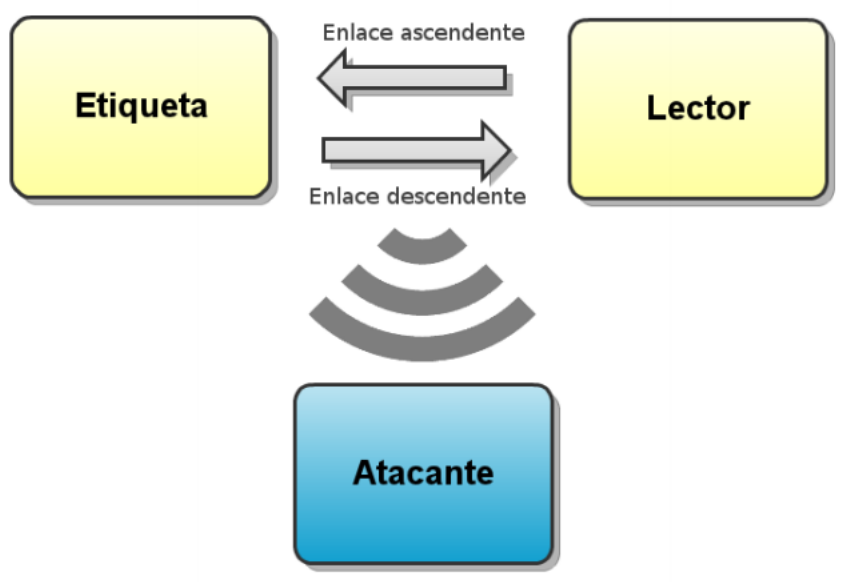
\includegraphics[width=0.5\textwidth]{figures/eavesdropping.png}
\end{figure}
\clearpage
El espiar (snooping) y el observar los paquetes en la red (sniffing) son términos comunes para el eavesdropping.

El eavesdropping es el escuchar una conversación, espiar, husmear. La información recolectada por eavesdropping se puede utilizar para planear otros ataques a la red.

Un ejemplo de los datos susceptibles al eavesdropping, son las secuencias utilizadas en las comunidades SNMP versión 1, ya que se envían en texto claro. Un intruso podría hacer eavesdropping en los intercambios de información de SNMP, y recopilar datos valiosos de la configuración del equipo de la red.

Otro ejemplo, es la captura de nombres de usuario y contraseñas, números de la tarjeta de crédito o información personal sensible, cuando cruzan una red.

Un método común para realizar eavesdropping en comunicaciones, es capturar paquetes TCP/IP o de otros protocolos y descifrar el contenido usando un analizador de protocolos o una utilidad similar.
%-----------
\subsection{Skimming}
Esta es la vulnerabilidad que atacaremos nosotros en el proyecto, consiste en obtener toda la información del sistema de la víctima y replicarlo en donde el atacante quiera. En esencia, la clonación.\\

\begin{figure}[!h]
	\centering
	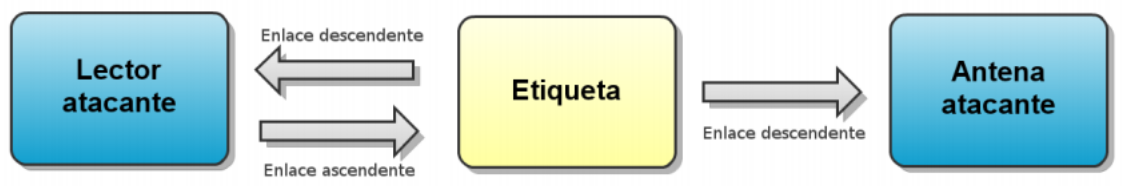
\includegraphics[width=0.5\textwidth]{figures/skimming.png}
\end{figure}
Los escenarios comunes en los que se realiza skimming es en restaurantes, bares, gasolineras o en cajeros electrónicos donde un cómplice del criminal está en posesión de la tarjeta de crédito de la víctima o en un lugar en el que se ha instalado un dispositivo que puede copiar la información.

En el caso de un cajero automático, el autor del fraude pone un disposan a menudo en combinación con una microcámara que graba el código PIN (Código de seguridad) del usuario.

Es difícil que el titular de la tarjeta detecte el skimming, pero es bastante fácil de detectar para el emisor de la tarjeta con una muestra lo suficientemente grande.

Por lo general, alguien en un cajero automático o en un local comercial utiliza un pequeño dispositivo para copiar y robar datos de la banda magnética de una tarjeta de crédito o de débito. Esa información se coloca sobre una tarjeta falsificada y se utiliza para hacer compras fraudulentas.
%-----------
\subsection{Denial of Service}
Como en muchas otras disciplinas, en el campo de las NFC también es posible hacerle a la víctima una denegación de servicio saturando el sistema y llenándolo de ruido.
\begin{figure}[!h]
	\centering
	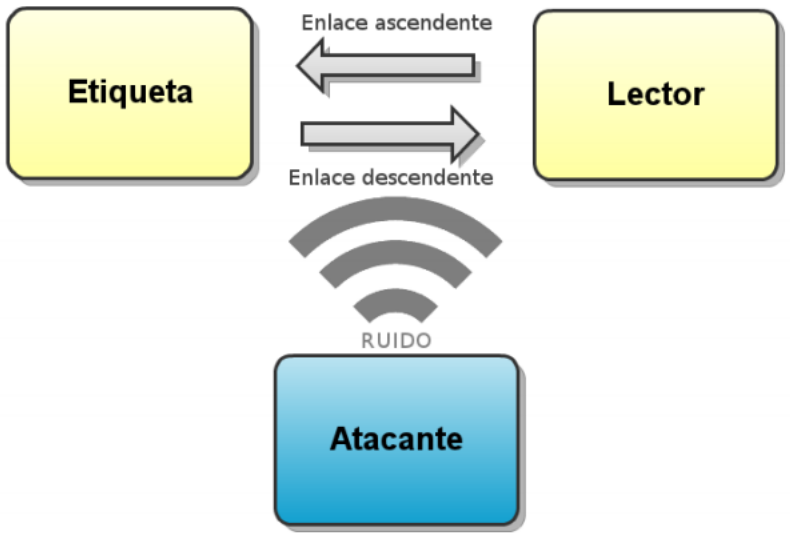
\includegraphics[width=0.4\textwidth]{figures/dos.png}
\end{figure}
%-----------
\subsection{Modificación de datos}
Este ataque consiste en modificar alguno -o todos- de los datos con los que actualmente cuenta la tarjeta. Esto puede utilizarse para el beneficio del sistema, por ejemplo recargar alguna tarjeta monedero, o para corromperla, insertando un chorro de unos.
\begin{figure}[!h]
	\centering
	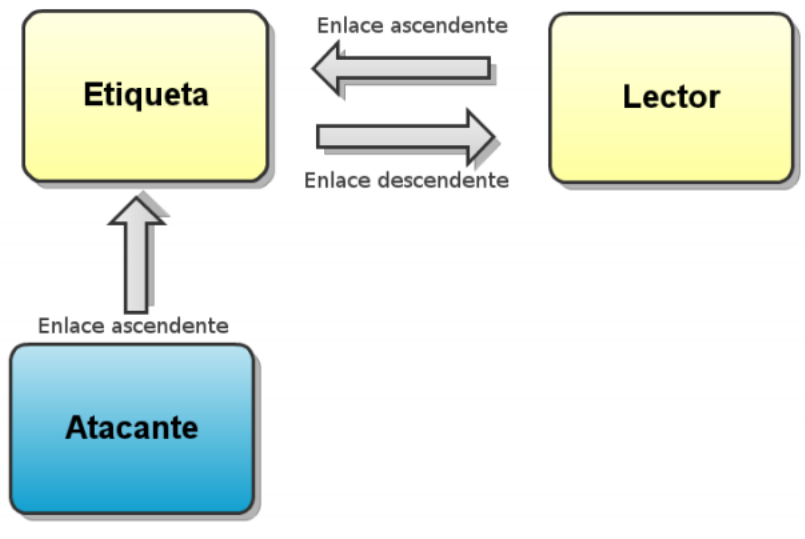
\includegraphics[width=0.4\textwidth]{figures/modificacion.png}
\end{figure}
\clearpage
%-----------
\subsection{Inserción de datos}
La inserción de datos se basa en sustituir el mensaje que la víctima manda por la que el atacante desee.
\begin{figure}[!h]
	\centering
	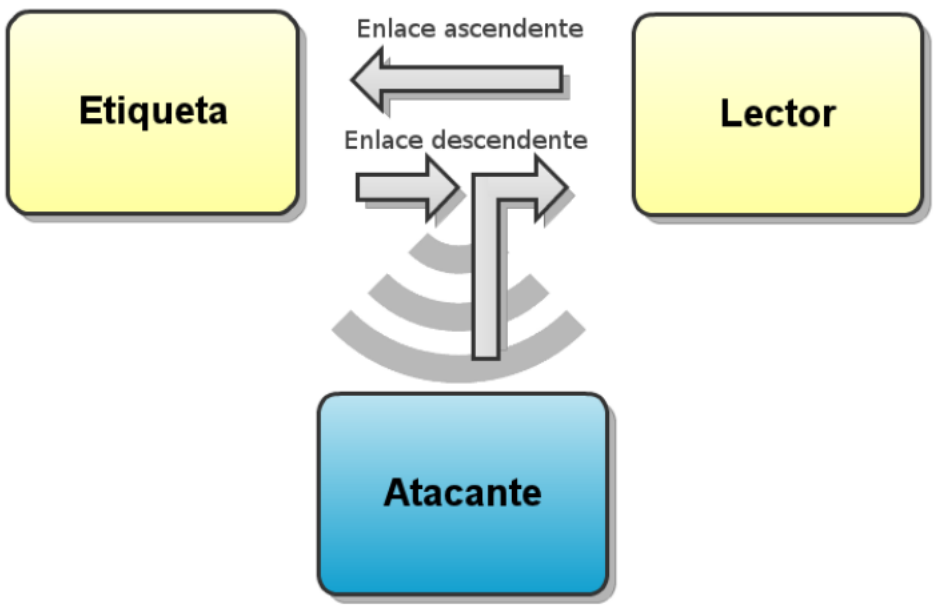
\includegraphics[width=0.5\textwidth]{figures/insercion.png}
\end{figure}
%-----------
\subsection{Man-in-the-middle}
En el proceso de man-in-the-middle se basa en interceptar los mensajes y después mandarlo modificados o igual que como la víctima los intercepta.
\begin{figure}[!h]
	\centering
	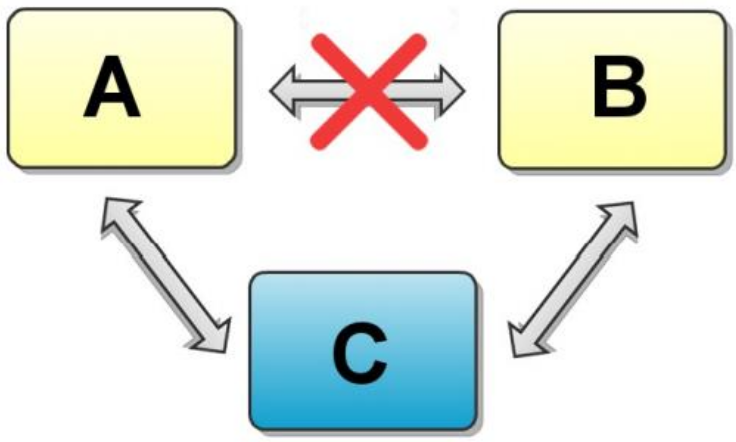
\includegraphics[width=0.5\textwidth]{figures/man.png}
\end{figure}


